\documentclass[11pt]{article}
\usepackage[spanish]{babel}
\usepackage[T1]{fontenc}
\usepackage{amsmath,amsfonts,amssymb,amsthm}
\usepackage{amsfonts}
\usepackage{graphicx}
\usepackage{geometry}
\usepackage{newpxtext,euler}
\usepackage{float}
\usepackage{xcolor}
\usepackage{geometry}
\usepackage{tikz}
 \geometry{
 a4paper,
 total={170mm,245mm},
 left=20mm,
 top=30mm,
 }
\pagestyle{empty}

\title{Taller III}

\author{Bourbaki}
\date{\today}


\begin{document}

\maketitle


\begin{enumerate}
    \item Demuestre que \( A \subset \mathbb{C} \) es compacto si y solo si es acotado y cerrado.

    \begin{proof}
    Supongamos que $A$ es compacto, si $A$ no es acotado entonces para todo $n\in \mathbb{N}$, existe $z_n\in A$ tal que $|z_n|>n$, por tanto $\{z_n\}$ no tiene punto de acumulación ya que... suponga que $z_0$ es un punto de acumulación, sea $m>2|z_0|$, es claro que $|z_0|>0$ ya que en caso contrario $z_0=0$, así pues $|z_n-z_0|=|z_n|>n$ y por lo tanto $z_0$ no sería punto de acumulación. En este caso $|z_m-z_0|\geq |z_m|-|z_0|>2|z_0|-|z_0|=|z_0|$, contradice que ese coso es punto límite. Entonces es acotado.\\

    Sea $z_0\in \overline{A}$, dado $n$, existe $z_n\in A$ tal que $|z_n-z_0|<\dfrac{1}{n}$, así $\{z_n\}$ converge a $z_0$. Como $A$ es compacto existe una subsucesión convergente en A, es claro que este límite debe ser $z_0$, así $z_0\in A$, con lo cual $A$ es cerrado.\\

    Recíprocamente, sea $\{z_n\}=\{x_n\}+i\{y_n\}\subseteq A$ , entonces existe un $M>0$ tal que $|z_n|\leq M$ para todo $n$, en particular $\{x_n\}\leq M$ y $\{y_n\}\leq M$ por lo tanto tienen una subsucesión convergente ya que son sucesiones de números reales, digamos $\{x_{n_1}\}\to a$ y $\{y_{n_2}\}\to b$, aplicamos el teorema de Bolzano en $\mathbb{R}$, esto es $z_n$ tiene una subsucesión convergente a $a+bi$.
    \end{proof}

    \item Sea \( K \subset \mathbb{C} \) compacto. Sean \( K_1 \supseteq K_2 \supseteq K_3 \supseteq \cdots \) una sucesión de subconjuntos de \( K \) no vacíos, tales que \( K_n \supseteq K_{n+1} \). Demostrar que la intersección de todos los \( K_n, n = 1, 2, 3, \ldots \) es no vacía.\\

    Pues lo que pasa es que eso siempre es  fácil allí porque usted llega y coge el conjunto $\left(0,\dfrac{1}{n}\right)$ $n\in \mathbb{N}$, note que ese conjunto está contenido en $[0,1]$ que es compacto, y pues si usted considera la intersección de esos coyos, eso le da vacío siono?

    \item Encontrar la imagen de las regiones:
    \[1 < | \operatorname{Im}(z) | \leq 2\]

    \begin{figure}[H]
    \centering
    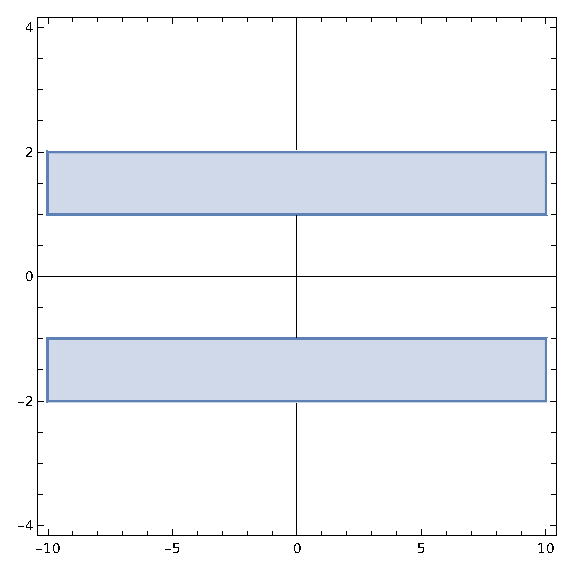
\includegraphics[scale=0.8]{Graphics/P3-1.eps}
    \end{figure}

    \[|z| < 1\]

    \begin{figure}[H]
    \centering
    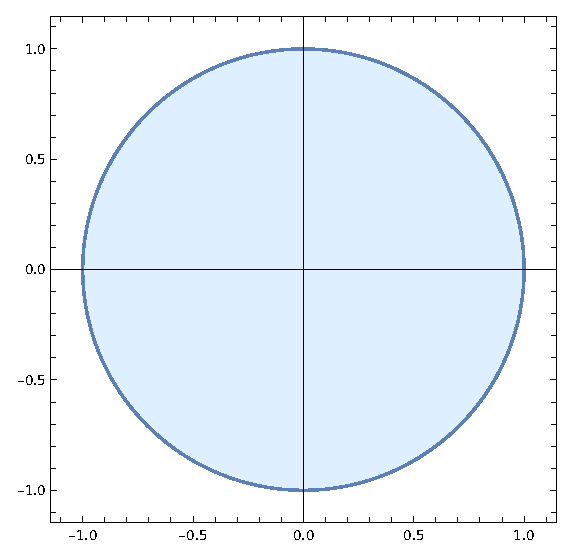
\includegraphics[scale=0.8]{Graphics/P3-2.eps}
    \end{figure}

    bajo las aplicaciones:
    \begin{enumerate}
        \item \( f(z) = z^2 \)\\

        Sea $z=x+yi$, entonces $z^2=x^2-y^2+2xyi$, sean $u(x,y)=x^2-y^2$ y $v(x,y)=2xy$ las funciones parte real e imaginaria, esto es

        $$x=\frac{v}{2y}$$ 

        reemplazando en la ecuación de arriba se obtiene que 

        $$u=\frac{v^2}{4y^2}-y^2$$

        si uno reemplaza en $-2$ y $-1$ obtiene las ecuaciones de dos parábolas, pero pues usted tiene que girar la cabeza  para verlo bien

        $$u=\frac{v^2}{16}-4\quad u=\frac{v^2}{4}-1$$

       \begin{figure}[H]
        \centering
        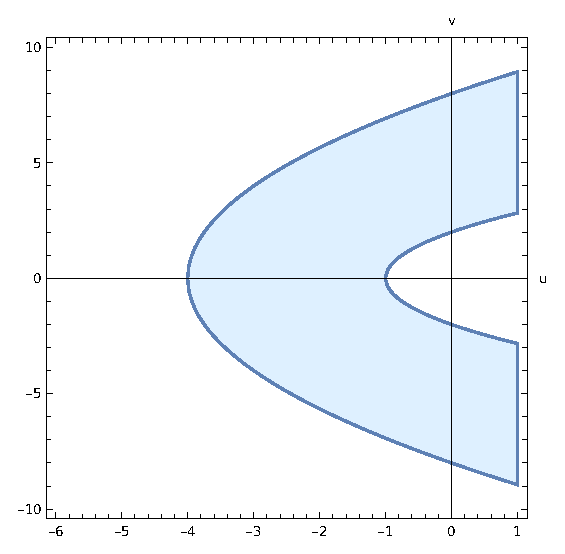
\includegraphics[scale=0.86]{Graphics/S1.eps}
        \end{figure}     

        Para el caso $|z|<1$ nos deja la misma bola porque dado $z=re^{i\theta}$ entonces $z^2=r^2e^{i2\theta}$ por lo que nos queda la misma circunferencia, dado que si $0\leq r<1$ entonces $0\leq r^2<1$
        \item \( f(z) = \dfrac{2z + i}{z + 1} \)\\

        \textcolor{red}{Esto lo irá a hacer su madre y con su madre me refiero al Santiago xd.}

    \end{enumerate}

    \item  Sea \( f(z) = \dfrac{z - i}{z + i} \), hallar la imagen por \( f \) de:
    \begin{enumerate}
        \item El semiplano superior.\\

        \item La semirecta \( it; t \geq 0 \).
        \item La recta \( it; t \in \mathbb{R} \).
        \item \( |z - 1| = 1 \).
        \item \( |z| = 2; \operatorname{Im}(z) \geq 0 \).
    \end{enumerate}

    \item Sea \( A = \{ z \in \mathbb{C} : -\infty < \operatorname{Im}(z) \leq \alpha \} \). Si \( f(z) = e^z \), hallar \( f(A) \).

    \item Sea \( A = \{ z \in \mathbb{C} : |\operatorname{Re}(z)| < \frac{\pi}{2}, \operatorname{Im}(z) > 0 \} \). Si \( f(z) = \sin(z) \), hallar \( f(A) \).

    \item Determine completamente la proyección estereográfica (que lleva la esfera de Riemann en el plano complejo). Es decir, hallar explícitamente \( T \) y \( T^{-1} \).\\

Primero que todo hagamos el muñeco

\begin{center} 
\tikzset{every picture/.style={line width=0.75pt}} %set default line width to 0.75pt        

\begin{tikzpicture}[x=0.75pt,y=0.75pt,yscale=-1.6,xscale=1.6]
%uncomment if require: \path (0,300); %set diagram left start at 0, and has height of 300

%Straight Lines [id:da3784688136862797] 
\draw    (309.33,160.33) -- (413.6,160.98) ;
\draw [shift={(416.6,161)}, rotate = 180.36] [fill={rgb, 255:red, 0; green, 0; blue, 0 }  ][line width=0.08]  [draw opacity=0] (5.36,-2.57) -- (0,0) -- (5.36,2.57) -- cycle    ;
%Straight Lines [id:da23548119284178148] 
\draw  [dash pattern={on 4.5pt off 4.5pt}]  (309.33,160.33) -- (309.15,61) ;
\draw [shift={(309.14,58)}, rotate = 89.89] [fill={rgb, 255:red, 0; green, 0; blue, 0 }  ][line width=0.08]  [draw opacity=0] (5.36,-2.57) -- (0,0) -- (5.36,2.57) -- cycle    ;
%Shape: Circle [id:dp3375096436146432] 
\draw   (250,155.3) .. controls (250,121.67) and (277.27,94.4) .. (310.9,94.4) .. controls (344.53,94.4) and (371.8,121.67) .. (371.8,155.3) .. controls (371.8,188.93) and (344.53,216.2) .. (310.9,216.2) .. controls (277.27,216.2) and (250,188.93) .. (250,155.3) -- cycle ;
%Shape: Ellipse [id:dp7427888218228516] 
\draw  [dash pattern={on 4.5pt off 4.5pt}] (250.33,160.33) .. controls (250.33,155.25) and (277.37,151.13) .. (310.73,151.13) .. controls (344.09,151.13) and (371.13,155.25) .. (371.13,160.33) .. controls (371.13,165.41) and (344.09,169.53) .. (310.73,169.53) .. controls (277.37,169.53) and (250.33,165.41) .. (250.33,160.33) -- cycle ;
%Straight Lines [id:da32292285281180777] 
\draw    (308.8,94.8) -- (375.66,223.4) ;
%Shape: Ellipse [id:dp12198761097569122] 
\draw  [dash pattern={on 0.84pt off 2.51pt}] (357.68,206.79) .. controls (357.68,203.54) and (361.83,200.92) .. (366.94,200.92) .. controls (372.05,200.92) and (376.2,203.54) .. (376.2,206.79) .. controls (376.2,210.03) and (372.05,212.66) .. (366.94,212.66) .. controls (361.83,212.66) and (357.68,210.03) .. (357.68,206.79) -- cycle ;
%Shape: Ellipse [id:dp535189966605516] 
\draw  [dash pattern={on 0.84pt off 2.51pt}] (316.98,123.45) .. controls (316.98,118.48) and (319.82,114.45) .. (323.32,114.45) .. controls (326.83,114.45) and (329.67,118.48) .. (329.67,123.45) .. controls (329.67,128.42) and (326.83,132.45) .. (323.32,132.45) .. controls (319.82,132.45) and (316.98,128.42) .. (316.98,123.45) -- cycle ;
%Shape: Circle [id:dp8877662772415491] 
\draw  [draw opacity=0][fill={rgb, 255:red, 74; green, 144; blue, 226 }  ,fill opacity=1 ] (321.82,123.45) .. controls (321.82,122.64) and (322.47,121.99) .. (323.28,121.99) .. controls (324.09,121.99) and (324.75,122.64) .. (324.75,123.45) .. controls (324.75,124.26) and (324.09,124.92) .. (323.28,124.92) .. controls (322.47,124.92) and (321.82,124.26) .. (321.82,123.45) -- cycle ;
%Shape: Ellipse [id:dp24083031390440834] 
\draw  [draw opacity=0][fill={rgb, 255:red, 74; green, 144; blue, 226 }  ,fill opacity=1 ] (364.94,206.79) .. controls (364.94,205.71) and (365.83,204.84) .. (366.94,204.84) .. controls (368.05,204.84) and (368.95,205.71) .. (368.95,206.79) .. controls (368.95,207.86) and (368.05,208.74) .. (366.94,208.74) .. controls (365.83,208.74) and (364.94,207.86) .. (364.94,206.79) -- cycle ;
%Straight Lines [id:da18519386133814764] 
\draw    (309.33,160.33) -- (240.88,218.65) ;
\draw [shift={(238.6,220.6)}, rotate = 319.57] [fill={rgb, 255:red, 0; green, 0; blue, 0 }  ][line width=0.08]  [draw opacity=0] (5.36,-2.57) -- (0,0) -- (5.36,2.57) -- cycle    ;
%Shape: Circle [id:dp24266992012860777] 
\draw  [draw opacity=0][fill={rgb, 255:red, 255; green, 0; blue, 0 }  ,fill opacity=1 ] (307.53,160.33) .. controls (307.53,159.34) and (308.34,158.53) .. (309.33,158.53) .. controls (310.33,158.53) and (311.13,159.34) .. (311.13,160.33) .. controls (311.13,161.33) and (310.33,162.13) .. (309.33,162.13) .. controls (308.34,162.13) and (307.53,161.33) .. (307.53,160.33) -- cycle ;
%Shape: Circle [id:dp8186682700140651] 
\draw  [draw opacity=0][fill={rgb, 255:red, 65; green, 117; blue, 5 }  ,fill opacity=1 ] (307.3,94.4) .. controls (307.3,93.41) and (308.11,92.6) .. (309.1,92.6) .. controls (310.09,92.6) and (310.9,93.41) .. (310.9,94.4) .. controls (310.9,95.39) and (310.09,96.2) .. (309.1,96.2) .. controls (308.11,96.2) and (307.3,95.39) .. (307.3,94.4) -- cycle ;

% Text Node
\draw (315.2,83.6) node [anchor=north west][inner sep=0.75pt]  [font=\tiny]  {$N=( 0,0,1)$};
% Text Node
\draw (331.67,117.4) node [anchor=north west][inner sep=0.75pt]  [font=\tiny]  {$(\hat{x} ,\hat{y} ,\hat{z})$};
% Text Node
\draw (391,201.07) node [anchor=north west][inner sep=0.75pt]  [font=\scriptsize]  {$( x,y,0) =( x,y) =z$};
\end{tikzpicture}
    \end{center}

    El vector director de la recta es $D=(x,y,0)-N=(x,y,-1)$, entonces la recta es

    $$(\hat{x},\hat{y},\hat{z})=(0,0,1)+t(x,y,-1)\quad t\geq 0$$

    de esto se sigue que

    $$\begin{cases}
    \hat{x}=tx\\
    \hat{y}=ty\\
    \hat{z}=1-t.
    \end{cases}$$

    Reemplazando esto en la ecuación de la esfera obtenemos $(tx)^2+(ty)^2+(1-t)^2=1$, esto es $t^2(x^2+y^2+1)=2t$, esto es $t=\dfrac{2}{x^2+y^2+1}$, reemplazando en las ecuaciones de antes se sigue que

    $$\begin{cases}
    \hat{x}=\dfrac{2x}{x^2+y^2+1}\\
    \\
    \hat{y}=\dfrac{2y}{x^2+y^2+2}\\
    \\
    \hat{z}=\dfrac{x^2+y^2-1}{x^2+y^2+1}
    \end{cases}$$

Por otro lado $t=1-\hat{z}$, esto es $x=\dfrac{\hat{x}}{1-\hat{z}}$, $y=\dfrac{\hat{y}}{1-\hat{z}}$, con esto podemos definir los mapeos:

\begin{align*}
    T:\quad&S\mapsto C\cup \{\infty\}=\widetilde{\mathbb{C}}\\
    &(\hat{x},\hat{y},\hat{z})\mapsto\left(\frac{\hat{x}}{1-\hat{z}},\frac{\hat{y}}{1-\hat{z}}\right)\\
    T^{-1}:\quad&\widetilde{\mathbb{C}}\mapsto S\\
    &\infty\to (0,0,1)\\
    &(\hat{x},\hat{y},\hat{z})\mapsto\left(\frac{2x}{x^2+y^2+1},\frac{2y}{x^2+y^2+1},\frac{x^2+y^2-1}{x^2+y^2+1}\right)
.\end{align*}

    \item Demostrar que la proyección estereográfica preserva círculos. La imagen directa o inversa de una circunferencia es una circunferencia.

    \begin{proof}
   Dada $A(x^2+y^2)+Bx+Cy+D=0$ la ecuación de la circunferencia, tenemos que $\hat{x}^2+\hat{y}^2=1-\hat{z}^2$, esto nos da que

   \begin{align*}
       0&=A\left(\frac{\hat{x}^2}{(1-\hat{z})^2}+\frac{\hat{y}^2}{(1-\hat{z})^2}\right)+B\frac{\hat{x}}{1-\hat{z}}+C\frac{\hat{y}}{1-\hat{z}}+D\\
       &=A\left(\frac{1-\hat{z}^2}{(1-\hat{z})^2}\right)+B\frac{\hat{x}}{1-\hat{z}}+C\frac{\hat{y}}{1-\hat{z}}+D\\
       &=\frac{1}{1-\hat{z}}\left(A(1+\hat{z})+B\hat{x}+C\hat{y}+D(1-\hat{z})\right)
   .\end{align*}

   Esto da que una circunferencia en $\mathbb{C}$ la envía en una circunferencia en $S$, una recta en $\mathbb{C}$ la manda en una circunferencia que pasa por el polo $N$. Recíprocamente si $(\hat{x},\hat{y},\hat{z})\in  S$, como $\hat{x}^2+\hat{y}^2+\hat{z}^2=1$ y $D=R^2-(A^2+B^2+C^2)$, entonces \textcolor{red}{aquí yo no entiendo de donde sale esa ecuación D, pero pues luego les pregunto xd}

   $$\hat{x}^2+\hat{y}^2+\hat{z}^2-2B\hat{y}-2C\hat{z}-D=0$$

   reemplazando los valores de $\hat{x}$, $\hat{y}$ y $\hat{z}$ se obtiene la ecuación 

   $$
\left(x^2+y^2\right)(1-2C-D)-4 A x-4 B y+(1+2 C-D)=0 .
$$

Y eso es una circunferencia en $\mathbb{C}$ a menos que $1-2C-D=0$ y eso es si la circunferencia pasa por el polo, en ese caso da una recta y fechó. \textcolor{red}{me toca creer unas cosas porque yo no me sé las ecuaciones de esas vainas}
\end{proof}

\end{enumerate}

\end{document}